\documentclass[slovak]{iamthesis}
% changle "slovak" to "english" for english version of the thesis

%----------------------------------------------------------------%
% THESIS DATA

% student name with title e.g. Ing. Martin Klaučo
\def\thesisauthor{Meno študenta} 

% year of submmiting to AIS
\def\thesisyear{rok}

% registration number generated by AIS e.g. 19990-50920
\def\thesisnumber{číslo práce} 

% thesis type: BACHELOR|MASTER|DISSERTATION or in slovak 
% BAKALÁRSKA|DIPLOMOVÁ|DIZERTAČNÁ
\def\thesistype{DIPLOMOVÁ}

% thesis title
\def\thesistitle{Názov práce}

% thesis supervisor including degrees e.g. Ing. Martin Klaučo, PhD.
\def\thesissupervisor{Ing. Martin Klaučo, PhD.}

% study field (translate to english if neccesarry) e.g. "Riadenie Procesov" or
% "Process Control"
\def\thesisprogram{Riadenie Procesov}

% Institute (translate to english if neccesary)
% e.g., "Institute of Information Engineering, Automation, and Mathematics"
\def\thesisinst{Ústav Automatizácie, Informatizácie a Riadenia Procesov}

% Title of the Acknowledgment
% For slovak write: "Poďakovanie" for English write: "Acknowledgment"
\def\thesisack{Poďakovanie}


% End THESIS DATA
%----------------------------------------------------------------%

%----------------------------------------------------------------%
%   Titles and other stuff                                       %
%----------------------------------------------------------------%
\author{\thesisauthor}
\title{\thesistitle}
\date{\today}
%\usepackage{layouts}
%\usepackage{layout}
%----------------------------------------------------------------%
%   Let the document begin                                       %
%----------------------------------------------------------------%
\begin{document}

% ---------------------------------------------------------------%
% The Frontmatter  !! Do NOT change the structure !!             % 
%----------------------------------------------------------------%

\coverpage

\frontmatter
\pagenumbering{roman}

% include assignment generated by AIS system
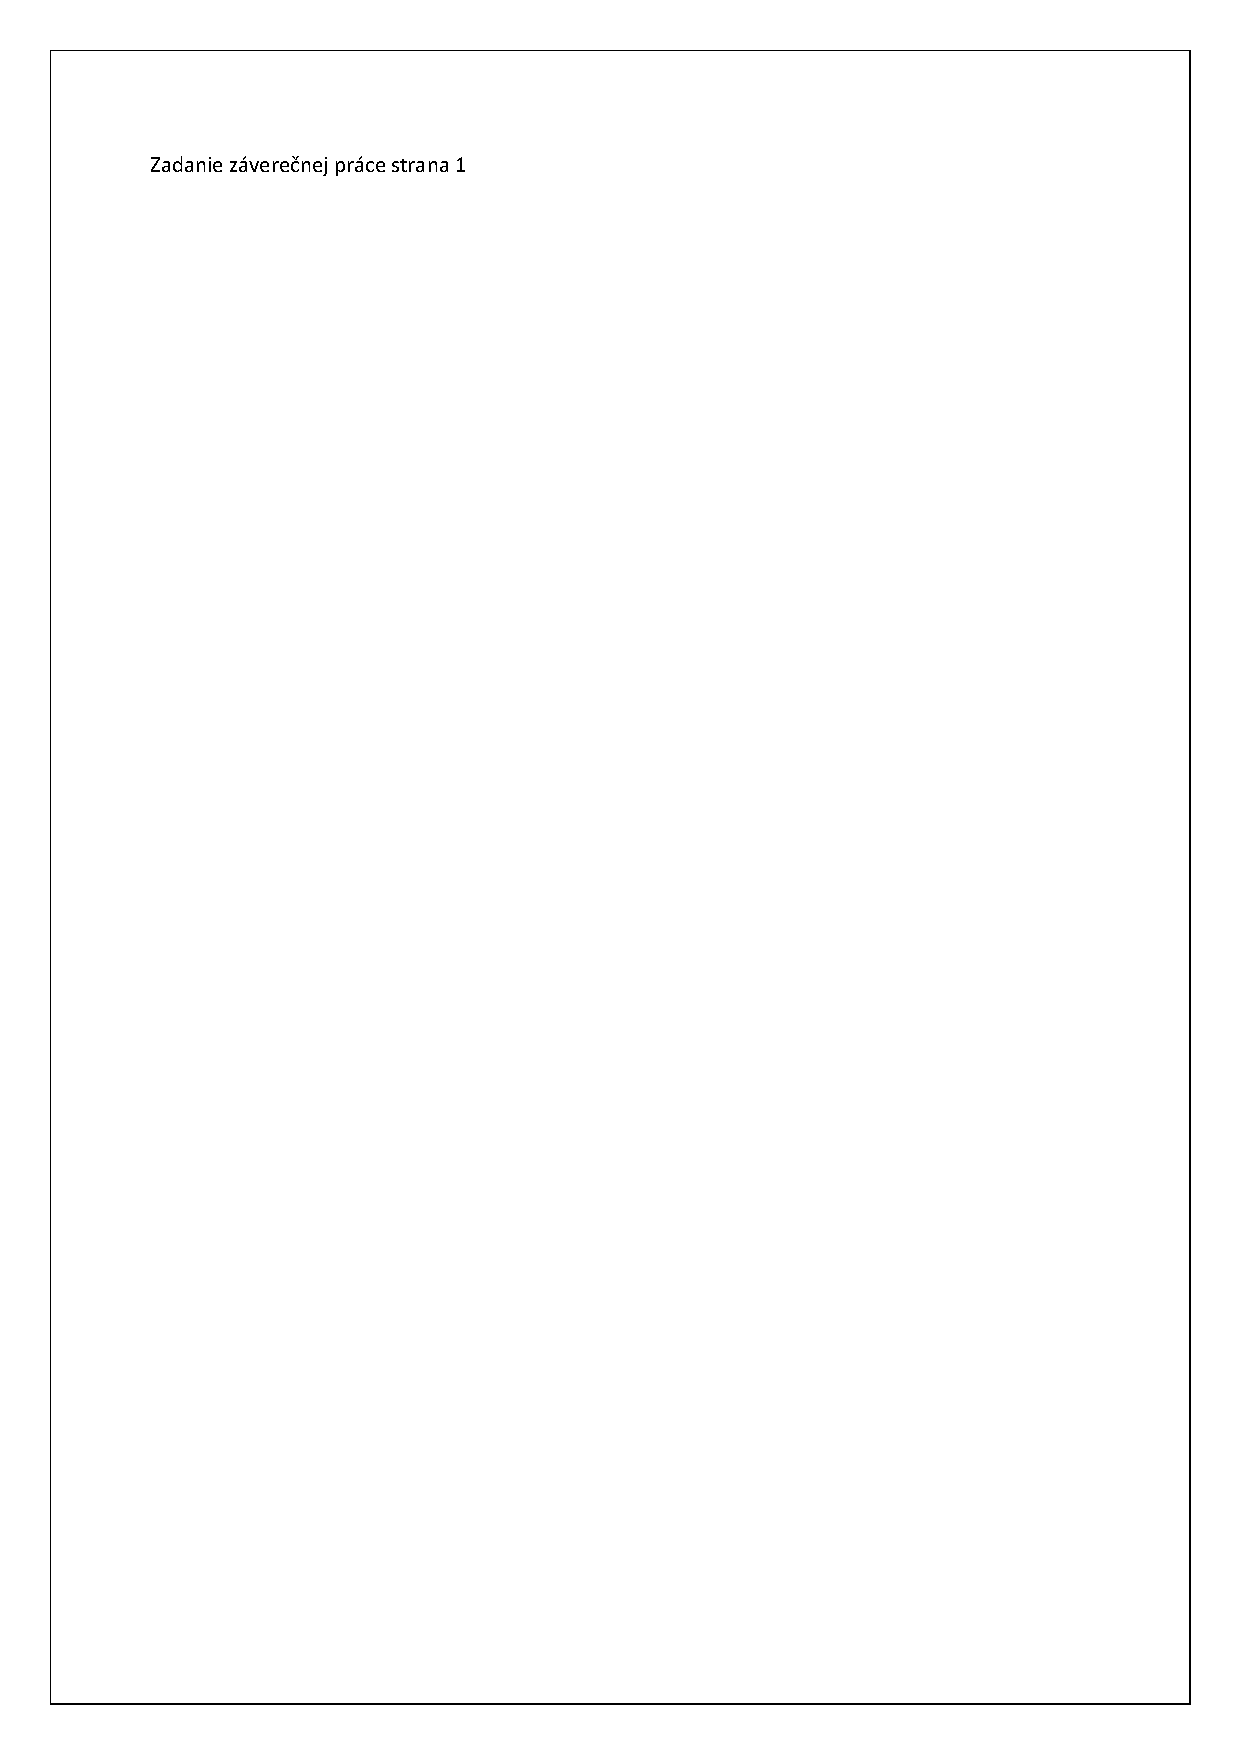
\includepdf[page=1]{content/assignment.pdf}
% use this command only if your assignment has more than 2 pages
% 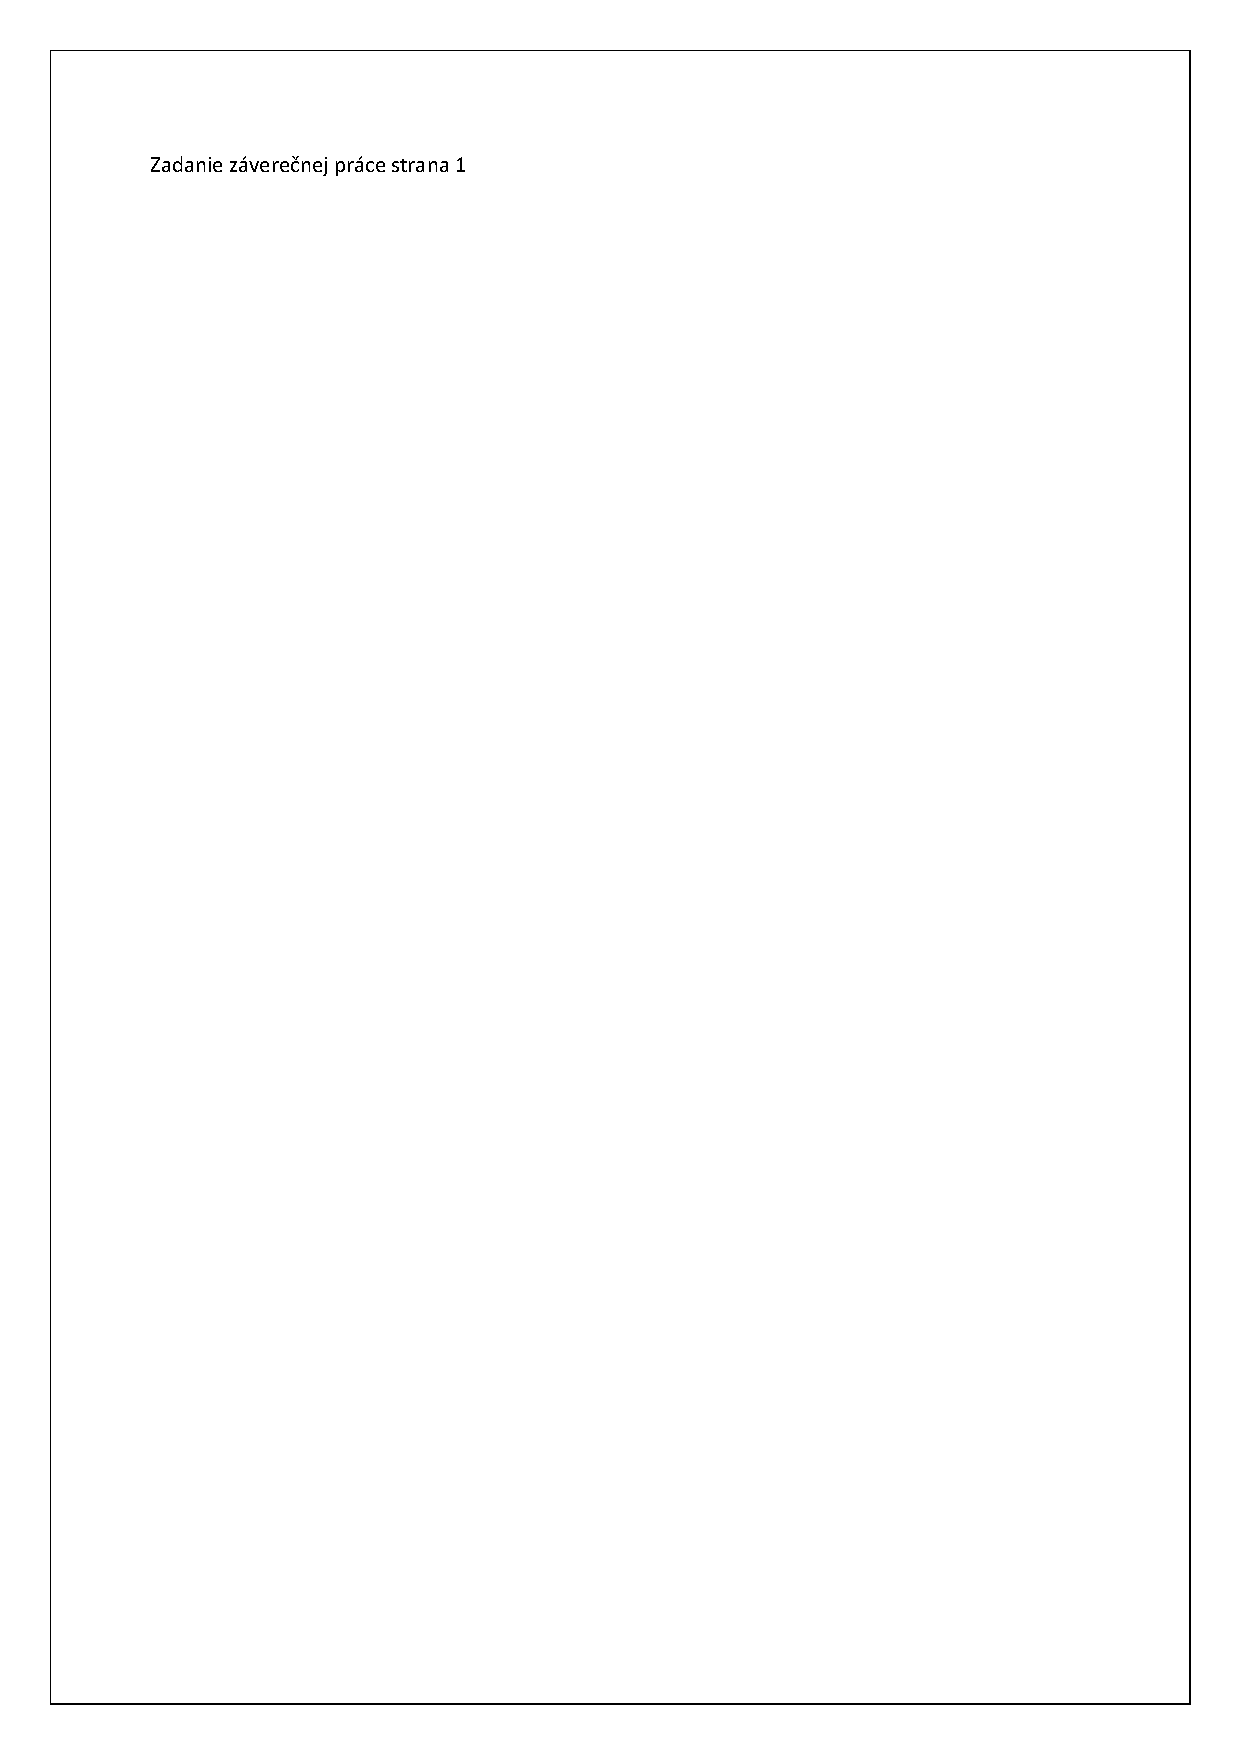
\includepdf[page=2]{content/assignment.pdf}


% do not remove following commands
% do not following commands
\chapter*{\thesisack}
\markboth{}{}
\addcontentsline{toc}{chapter}{\thesisack}
Write here the acknowledgment

\chapter*{Abstract}
\markboth{}{}
\addcontentsline{toc}{chapter}{Abstract}
English abstract

\chapter*{Abstrakt}
\markboth{}{}
\addcontentsline{toc}{chapter}{Abstrakt}
Slovenský abstrakt

\setcounter{tocdepth}{2}
\renewcommand{\baselinestretch}{0.1}\normalsize
\tableofcontents
\renewcommand{\baselinestretch}{1.1}\normalsize

% ----------------------------------------------------------------%
% The Mainmatter !! Do NOT change the structure!!                 %
% ----------------------------------------------------------------%
\mainmatter

% individual chapters should be included via a separate tex file, as shown in 
% here. When working in TexStudio (recomennded tool for Win and Mac) set the 
% main.tex as an Explicit root document, so you can compile even you are
% working on other chapter in other tex file.
%
% Open main.tex THEN click Options-> Root Document -> Set Current Document as
% Explicit Root

% introduction
\chapter{Introduction}
\label{ch:intro}

This \LaTeX template is intended for student writing their final theses at 
Faculty of Chemical and Food Technology. This chapter covers the basic setup of 
the LaTeX template as well as simple guidelines for high-quality typesetting. 
This template generates the thesis structure based on requirements. The 
template is intended for Slovak-writing as well as for English-writing students
\begin{verbatim}
\documentclass[english]{iamthesis}
% changle "english" to "slovak" for english version of the thesis
\end{verbatim}

The file structure of this LaTeX template
\begin{verbatim}
	|-- content/
	   |-- abstract_en.tex
	   |-- abstract_sk.tex
	   |-- introduction.tex	   
	   |-- assignment.pdf
	   |-- theory.tex
	   |-- conclusions.tex
	   |-- resume.tex
	|-- images/
		 |-- fchpt_logo_color.pdf
	|-- main.tex
	|-- bibfile.bib
\end{verbatim}

The root document is the \texttt{main.tex}. Here, the student must specify 
key-values of the thesis (lines 7 to 32), namely:
\begin{verbatim}
% student name with title e.g. Ing. Martin Klaučo
\def\thesisauthor{Students Name} 

% year of submmiting to AIS
\def\thesisyear{Year}

% registration number generated by AIS e.g. 19990-50920
\def\thesisnumber{Number} 

% thesis type: BACHELOR|MASTER|DISSERTATION or in slovak 
% BAKALÁRSKA|DIPLOMOVÁ|DIZERTAČNÁ
\def\thesistype{DIPLOMOVÁ}

% thesis title
\def\thesistitle{Title of the Thesis}

% thesis supervisor including degrees e.g. MSc. Ing. Martin Klaučo, PhD.
\def\thesissupervisor{Ing. Martin Klaučo, PhD.}

% study field (translate to english if neccesarry) e.g. 
% "Riadenie Procesov" or "Process Control"
\def\thesisprogram{Riadenie Procesov}

% Institute (translate to english if neccesary)
% e.g., "Institute of Information Engineering, Automation, and Mathematics"
\def\thesisinst{Ústav Automatizácie, Informatizácie a Riadenia Procesov}
\end{verbatim}

The file \texttt{assignment.pdf} is to be replaced by assignment generated by 
the AIS system.

The file \texttt{bibfile.bib} is to be expanded with your references. You can 
also provide your own bibfile. See command 
\texttt{\textbackslash{providebibliography}}.

\section{Typesetting Guidelines}
This template comes with predefined macros, help to ease up the typesetting of 
math. Refer to table~\ref{tab:commands} for examples.


Before submitting the thesis check if
\begin{itemize}
	\item all equations are referenced in the text (remember, you can refer only 
	to equation which was already written),
	\item all figures are referenced in the text (remember, figure must not 
	appear necessarily on the same page as you would like),
	\item all tables are referenced in the text (remember, figure must not 
		appear necessarily on the same page as you would like),
	\item every chapter, section or subsection must start with a paragraph,
	\item every chapter, section or subsection must end with text, not with 
	equation, nor with table or figure,
	\item if writing in English, check you grammar with free tool 
	\url{www.grammarly.com}.
\end{itemize}


\begin{table}[h]
	\centering
	\caption{Example of built-in commands}
	\label{tab:commands}
	\begin{tabular}{llp{5cm}}
		\toprule
			command & results & remark\\
		\midrule
		  \texttt{\textbackslash{ui\{F\}\{a\}}} &  $\ui{F}{a}$ & is used 
		  when the subindex ''a'' is part 
		  of notation\\
		  \texttt{\textbackslash{uis\{F\}\{a\}\{k\}}} &  $\uis{F}{a}{k}$ & is 
		  used  when  the  subindex ''a'' is  part  of notation and ''k'' is 
		  variable 
		  \\
		  \texttt{\textbackslash{Ts}} & $\Ts$ & sampling time \\[2pt]
		  \texttt{\textbackslash{lrp\{ \textbackslash{frac\{a\}\{b\}} \}}} & 
		  $\displaystyle\lrp{\frac{a}{b}}$& 
		  expandable parenthesis based on 
		  the expression size\\
		  \texttt{\textbackslash{lrb\{ \textbackslash{frac\{a\}\{b\}} \}}} & 
		  $\displaystyle\lrb{\frac{a}{b}}$& 
		  expandable brackets based on 
		  the expression size\\
		  \texttt{\textbackslash{diff\{f(x)\}\{x\}}} & 
		  $\displaystyle\diff{f(x)}{x}$& \\[10pt]
		  \texttt{\textbackslash{diffxy\{f(x,y)\}\{x\}\{y\}}} & 
		  $\displaystyle\diffxy{f(x, y)}{x}{y}$& \\[10pt]
		  \texttt{\textbackslash{diffxy\{f(x,y)\}\{x\}\{y\}}} & 
		  $\displaystyle\diffat{f(x, y)}{x}{x=0}$& \\[10pt]
		  \texttt{\textbackslash{dt\{f(t)\} } } & $\displaystyle\dt{f(t)}$  & \\
		\bottomrule
	\end{tabular}
	% the "\displaystyle" command for increased font size of the math expression 
	%  in table
\end{table}

Example of citing literature~\cite{boyd:book:2009:cvx}.

% theory
\chapter{Theory}

\section{First Section}
Some theory... 
\begin{equation}
	a^2 + b^2 = c^2
\end{equation}

\section{Second Section}
Lorem ipsum dolor sit amet, consectetur adipiscing elit. Praesent pulvinar 
lobortis justo, quis vulputate quam gravida id. Sed massa libero, fermentum at 
convallis a, fringilla at massa. Cras condimentum vel urna in accumsan. Morbi 
cursus risus eu magna efficitur rhoncus. Nullam tincidunt sit amet sapien non 
auctor. Morbi varius eros massa, nec tincidunt odio rhoncus et. Etiam sed orci 
sagittis, dapibus erat nec, venenatis velit. Ut malesuada, justo vel consequat 
ullamcorper, sem justo tristique purus, ac vulputate nulla lorem eu metus. In 
convallis orci mi, a varius est blandit a. Cras non gravida turpis, elementum 
molestie nisl. Duis in blandit magna.

\subsection{A Subsection}
Lorem ipsum dolor sit amet, consectetur adipiscing elit. Praesent pulvinar 
lobortis justo, quis vulputate quam gravida id. Sed massa libero, fermentum at 
convallis a, fringilla at massa. Cras condimentum vel urna in accumsan. Morbi 
cursus risus eu magna efficitur rhoncus. Nullam tincidunt sit amet sapien non 
auctor. Morbi varius eros massa, nec tincidunt odio rhoncus et. Etiam sed orci 
sagittis, dapibus erat nec, venenatis velit. Ut malesuada, justo vel consequat 
ullamcorper, sem justo tristique purus, ac vulputate nulla lorem eu metus. In 
convallis orci mi, a varius est blandit a. Cras non gravida turpis, elementum 
molestie nisl. Duis in blandit magna.

Sed consequat odio at elementum mollis. Fusce lacinia vulputate magna, vel 
consequat justo sagittis sit amet. Vestibulum lorem lectus, aliquet vitae 
malesuada non, congue ac libero. Aliquam volutpat mi varius odio scelerisque, 
sed semper sem feugiat. Morbi mauris tellus, auctor vitae commodo id, bibendum 
ut ante. Maecenas condimentum mauris tellus, eu eleifend purus rhoncus non. 
Lorem ipsum dolor sit amet, consectetur adipiscing elit. Vestibulum ante ipsum 
primis in faucibus orci luctus et ultrices posuere cubilia Curae; Integer vel 
lorem vulputate magna faucibus aliquam. Donec in erat imperdiet, rutrum velit 
quis, tempor tortor. Maecenas aliquam ligula dolor, eu mollis ante tempor eget.

Interdum et malesuada fames ac ante ipsum primis in faucibus. In justo ligula, 
lacinia quis iaculis ac, ullamcorper eu metus. Donec nibh diam, elementum vitae 
leo non, lacinia faucibus eros. Nulla volutpat lacus et ante imperdiet 
interdum. Aliquam pretium urna a ullamcorper aliquam. Fusce fermentum lorem ac 
turpis feugiat pulvinar. Proin felis est, sodales eu pretium at, consequat at 
libero. Aliquam facilisis sapien non justo consectetur semper. Morbi rhoncus 
leo sit amet mattis ullamcorper.

\subsection{A Subsection with Figure}

Lorem ipsum dolor sit amet, consectetur adipiscing elit. Praesent pulvinar 
lobortis justo, quis vulputate quam gravida id. Sed massa libero, fermentum at 
convallis a, fringilla at massa. Cras condimentum vel urna in accumsan. Morbi 
cursus risus eu magna efficitur rhoncus. Nullam tincidunt sit amet sapien non 
auctor. Morbi varius eros massa, nec tincidunt odio rhoncus et. Etiam sed orci 
sagittis, dapibus erat nec, venenatis velit. Ut malesuada, justo vel consequat 
ullamcorper, sem justo tristique purus, ac vulputate nulla lorem eu metus. In 
convallis orci mi, a varius est blandit a. Cras non gravida turpis, elementum 
molestie nisl. Duis in blandit magna.

Sed consequat odio at elementum mollis. Fusce lacinia vulputate magna, vel 
consequat justo sagittis sit amet. Vestibulum lorem lectus, aliquet vitae 
malesuada non, congue ac libero. Aliquam volutpat mi varius odio scelerisque, 
sed semper sem feugiat. Morbi mauris tellus, auctor vitae commodo id, bibendum 
ut ante. Maecenas condimentum mauris tellus, eu eleifend purus rhoncus non. 
Lorem ipsum dolor sit amet, consectetur adipiscing elit. Vestibulum ante ipsum 
primis in faucibus orci luctus et ultrices posuere cubilia Curae; Integer vel 
lorem vulputate magna faucibus aliquam. Donec in erat imperdiet, rutrum velit 
quis, tempor tortor. Maecenas aliquam ligula dolor, eu mollis ante tempor eget.

Interdum et malesuada fames ac ante ipsum primis in faucibus. In justo ligula, 
lacinia quis iaculis ac, ullamcorper eu metus. Donec nibh diam, elementum vitae 
leo non, lacinia faucibus eros. Nulla volutpat lacus et ante imperdiet 
interdum. Aliquam pretium urna a ullamcorper aliquam. Fusce fermentum lorem ac 
turpis feugiat pulvinar. Proin felis est, sodales eu pretium at, consequat at 
libero. Aliquam facilisis sapien non justo consectetur semper. Morbi rhoncus 
leo sit amet mattis ullamcorper.
Lorem ipsum dolor sit amet, consectetur adipiscing elit. Praesent pulvinar 
lobortis justo, quis vulputate quam gravida id. Sed massa libero, fermentum at 
convallis a, fringilla at massa. Cras condimentum vel urna in accumsan. Morbi 
cursus risus eu magna efficitur rhoncus. Nullam tincidunt sit amet sapien non 
auctor. Morbi varius eros massa, nec tincidunt odio rhoncus et. Etiam sed orci 
sagittis, dapibus erat nec, venenatis velit. Ut malesuada, justo vel consequat 
ullamcorper, sem justo tristique purus, ac vulputate nulla lorem eu metus. In 
convallis orci mi, a varius est blandit a. Cras non gravida turpis, elementum 
molestie nisl. Duis in blandit magna.

Sed consequat odio at elementum mollis. Fusce lacinia vulputate magna, vel 
consequat justo sagittis sit amet. Vestibulum lorem lectus, aliquet vitae 
malesuada non, congue ac libero. Aliquam volutpat mi varius odio scelerisque, 
sed semper sem feugiat. Morbi mauris tellus, auctor vitae commodo id, bibendum 
ut ante. Maecenas condimentum mauris tellus, eu eleifend purus rhoncus non. 
Lorem ipsum dolor sit amet, consectetur adipiscing elit. Vestibulum ante ipsum 
primis in faucibus orci luctus et ultrices posuere cubilia Curae; Integer vel 
lorem vulputate magna faucibus aliquam. Donec in erat imperdiet, rutrum velit 
quis, tempor tortor. Maecenas aliquam ligula dolor, eu mollis ante tempor eget.

Interdum et malesuada fames ac ante ipsum primis in faucibus. In justo ligula, 
lacinia quis iaculis ac, ullamcorper eu metus. Donec nibh diam, elementum vitae 
leo non, lacinia faucibus eros. Nulla volutpat lacus et ante imperdiet 
interdum. Aliquam pretium urna a ullamcorper aliquam. Fusce fermentum lorem ac 
turpis feugiat pulvinar. Proin felis est, sodales eu pretium at, consequat at 
libero. Aliquam facilisis sapien non justo consectetur semper. Morbi rhoncus 
leo sit amet mattis ullamcorper.
Lorem ipsum dolor sit amet, consectetur adipiscing elit. Praesent pulvinar 
lobortis justo, quis vulputate quam gravida id. Sed massa libero, fermentum at 
convallis a, fringilla at massa. Cras condimentum vel urna in accumsan. Morbi 
cursus risus eu magna efficitur rhoncus. Nullam tincidunt sit amet sapien non 
auctor. Morbi varius eros massa, nec tincidunt odio rhoncus et. Etiam sed orci 
sagittis, dapibus erat nec, venenatis velit. Ut malesuada, justo vel consequat 
ullamcorper, sem justo tristique purus, ac vulputate nulla lorem eu metus. In 
convallis orci mi, a varius est blandit a. Cras non gravida turpis, elementum 
molestie nisl. Duis in blandit magna.

Sed consequat odio at elementum mollis. Fusce lacinia vulputate magna, vel 
consequat justo sagittis sit amet. Vestibulum lorem lectus, aliquet vitae 
malesuada non, congue ac libero. Aliquam volutpat mi varius odio scelerisque, 
sed semper sem feugiat. Morbi mauris tellus, auctor vitae commodo id, bibendum 
ut ante. Maecenas condimentum mauris tellus, eu eleifend purus rhoncus non. 
Lorem ipsum dolor sit amet, consectetur adipiscing elit. Vestibulum ante ipsum 
primis in faucibus orci luctus et ultrices posuere cubilia Curae; Integer vel 
lorem vulputate magna faucibus aliquam. Donec in erat imperdiet, rutrum velit 
quis, tempor tortor. Maecenas aliquam ligula dolor, eu mollis ante tempor eget.

Interdum et malesuada fames ac ante ipsum primis in faucibus. In justo ligula, 
lacinia quis iaculis ac, ullamcorper eu metus. Donec nibh diam, elementum vitae 
leo non, lacinia faucibus eros. Nulla volutpat lacus et ante imperdiet 
interdum. Aliquam pretium urna a ullamcorper aliquam. Fusce fermentum lorem ac 
turpis feugiat pulvinar. Proin felis est, sodales eu pretium at, consequat at 
libero. Aliquam facilisis sapien non justo consectetur semper. Morbi rhoncus 
leo sit amet mattis ullamcorper.
Lorem ipsum dolor sit amet, consectetur adipiscing elit. Praesent pulvinar 
lobortis justo, quis vulputate quam gravida id. Sed massa libero, fermentum at 
convallis a, fringilla at massa. Cras condimentum vel urna in accumsan. Morbi 
cursus risus eu magna efficitur rhoncus. Nullam tincidunt sit amet sapien non 
auctor. Morbi varius eros massa, nec tincidunt odio rhoncus et. Etiam sed orci 
sagittis, dapibus erat nec, venenatis velit. Ut malesuada, justo vel consequat 
ullamcorper, sem justo tristique purus, ac vulputate nulla lorem eu metus. In 
convallis orci mi, a varius est blandit a. Cras non gravida turpis, elementum 
molestie nisl. Duis in blandit magna.

Sed consequat odio at elementum mollis. Fusce lacinia vulputate magna, vel 
consequat justo sagittis sit amet. Vestibulum lorem lectus, aliquet vitae 
malesuada non, congue ac libero. Aliquam volutpat mi varius odio scelerisque, 
sed semper sem feugiat. Morbi mauris tellus, auctor vitae commodo id, bibendum 
ut ante. Maecenas condimentum mauris tellus, eu eleifend purus rhoncus non. 
Lorem ipsum dolor sit amet, consectetur adipiscing elit. Vestibulum ante ipsum 
primis in faucibus orci luctus et ultrices posuere cubilia Curae; Integer vel 
lorem vulputate magna faucibus aliquam. Donec in erat imperdiet, rutrum velit 
quis, tempor tortor. Maecenas aliquam ligula dolor, eu mollis ante tempor eget.

Interdum et malesuada fames ac ante ipsum primis in faucibus. In justo ligula, 
lacinia quis iaculis ac, ullamcorper eu metus. Donec nibh diam, elementum vitae 
leo non, lacinia faucibus eros. Nulla volutpat lacus et ante imperdiet 
interdum. Aliquam pretium urna a ullamcorper aliquam. Fusce fermentum lorem ac 
turpis feugiat pulvinar. Proin felis est, sodales eu pretium at, consequat at 
libero. Aliquam facilisis sapien non justo consectetur semper. Morbi rhoncus 
leo sit amet mattis ullamcorper.

\begin{figure}
	\centering
	
\includegraphics[width = 0.5\textwidth]{images/fchpt_logo_color}
	\caption{A figure caption.}
	\label{fig:label}
\end{figure}

Maecenas posuere maximus ipsum, eget laoreet risus malesuada faucibus. Nam 
tincidunt at diam quis vestibulum. Nullam a tortor vestibulum, pellentesque 
diam eu, venenatis neque. Duis id egestas lacus. Cras condimentum lorem sit 
amet posuere venenatis. Vestibulum ante ipsum primis in faucibus orci luctus et 
ultrices posuere cubilia Curae; Morbi convallis at ipsum vitae tincidunt. Proin 
vel massa eget ligula accumsan convallis vitae sit amet est. Aliquam nisl 
felis, pharetra non purus malesuada, convallis faucibus est. Nulla odio nisi, 
tempus sed rhoncus vitae, accumsan vel nisl. Nunc varius tincidunt felis, ut 
iaculis lectus volutpat vitae. Vivamus id lectus sit amet nulla volutpat 
congue. Nunc fermentum sem ac neque feugiat lobortis. In vestibulum, nisi a 
condimentum posuere, urna enim dapibus ex, in ultricies est enim hendrerit ex.

Duis feugiat ac elit id molestie. Nullam a massa viverra, ornare odio nec, 
tempor enim. Proin suscipit est at leo bibendum ultricies. Curabitur ornare 
malesuada suscipit. Vivamus mollis orci at ante pellentesque, eu feugiat eros 
finibus. Curabitur facilisis, velit quis aliquet molestie, nunc nibh facilisis 
orci, ut porttitor neque tellus eget quam. Vivamus sollicitudin, ex non egestas 
consequat, tortor nulla tempor ligula, eget facilisis lectus quam nec metus. 
Etiam ornare ornare varius. Nulla facilisi. Nunc facilisis dui eget metus 
dictum, eu maximus felis semper. Morbi non aliquam est.

% conclusions
\chapter{Resumé}
\label{ch:resume}

Resumé v slovenčine, v rozsahu približne 3 strán, sa píše v prípade, že 
záverečná práca ja napísaná v anglickom jazyku.

% Appendices (Prílohy) comment by "%" if not neccesary
\appendix
\chapter{Resumé}
\label{ch:resume}

Resumé v slovenčine, sa píše v prípade, že záverečná práca ja napísaná v 
anglickom jazyku. Rozsah resumé tvorí 5-10\% rozsahu diplomovej práce.

%----------------------------------------------------------------%
%  The Backmatter !! Do NOT change the structure!!               %
%----------------------------------------------------------------%
% Bibliography to TOC
% do not remove
\backmatter
\providebibliography
\bibliography{bibfile}

%----------------------------------------------------------------%
%   The end of the document                                      %
%----------------------------------------------------------------%
\end{document}
